\part[Clean Code \& TDD]{Clean Code \& Test-Driven Development}
\section{Clean Code}
\begin{frame}{Robert Cecil Martin aka Uncle Bob}
\begin{center}
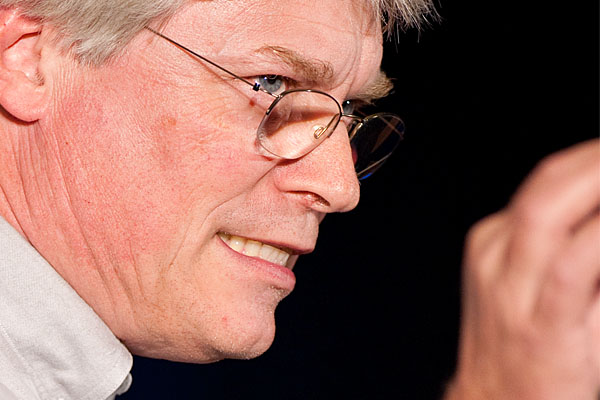
\includegraphics[width=0.7\textwidth]{resources/BobAtRails.jpg}\\
Uncle Bob is an award winning author, renowned speaker, and ueber software
geek since 1970. He is the founder and president of
\link{https://sites.google.com/site/unclebobconsultingllc/}{Uncle Bob
Consulting} and \link{http://www.objectmentor.com/}{Object Mentor}.
\end{center}
\end{frame}

\begin{frame}{Clean Code \& The Clean Coder}
\begin{columns}
	\column{.5\textwidth}
	\begin{center}
	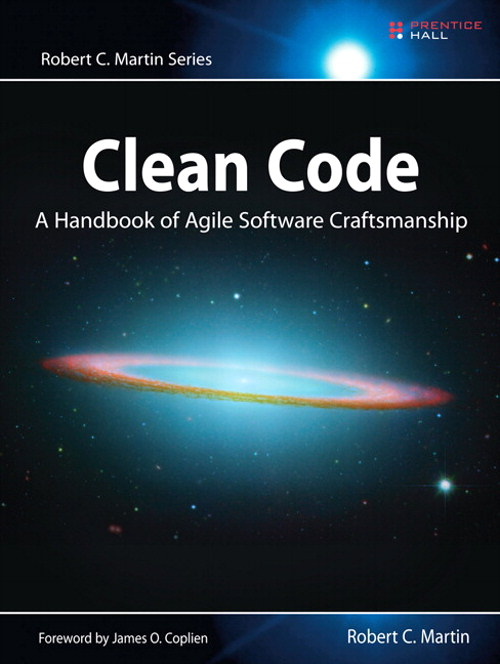
\includegraphics[width=0.8\textwidth]{resources/CleanCode.jpg}
	\end{center}
	\column{.5\textwidth}
	\begin{center}
	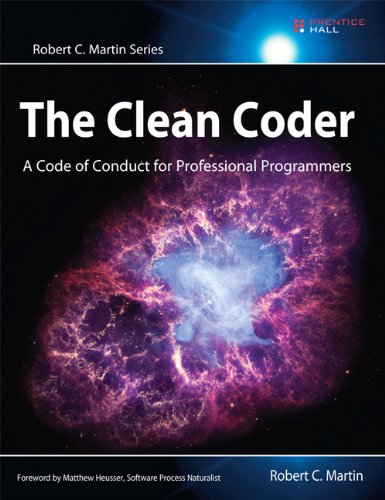
\includegraphics[width=0.8\textwidth]{resources/TheCleanCoder.jpg}
	\end{center}
\end{columns}
\end{frame}

\begin{frame}{There will always be code}
\begin{block}{The inconvenient truth}
Code matters, because there will always be code. Period.
\end{block}
\pause
\begin{block}{What is clean code?}
\pause
There is no such thing as clean code, there is only cleanable code
\end{block}
\pause
\begin{block}{What is cleanable code?}
Cleanable code is code with tests
\end{block}
\pause
\begin{block}{What is the boy scout rule?}
Leave the campground (the code base) cleaner than you found it
\end{block}
\end{frame}

\subsection{Meaningful Names}
\begin{frame}[fragile]{Meaningful Names}
\begin{alertblock}{Use intention-revealing names}
\begin{lstlisting}[language=java]
int d; // elapsed time in days
\end{lstlisting}
\end{alertblock}
\begin{exampleblock}{Use intention-revealing names}
\begin{lstlisting}[language=java]
int elapsedTimeInDays
\end{lstlisting}
\end{exampleblock}
\end{frame}

\begin{frame}[fragile]{Meaningful Names}
\begin{alertblock}{Avoid disinformation}
\lstinline!accountList!
\end{alertblock}
\begin{exampleblock}{Avoid disinformation}
\lstinline!accounts!
\end{exampleblock}
\end{frame}

\begin{frame}[fragile]{Meaningful Names}
\begin{alertblock}{Make meaningful distinctions}
\begin{lstlisting}[language=java]
getActiveAccount();
getActiveAccounts();
getActiveAccountInfo();
\end{lstlisting}
\end{alertblock}
\end{frame}

\begin{frame}[fragile]{Meaningful Names}
\begin{alertblock}{Use pronouncable Names}
\lstinline!class DtaRcrd102!
\end{alertblock}
\begin{exampleblock}{Use pronouncable Names}
\lstinline!class Customer!
\end{exampleblock}
\end{frame}

\begin{frame}[fragile]{Meaningful Names}
\begin{alertblock}{Use searchable names}
\lstinline!class Person(i: Int)!
\end{alertblock}
\center{The length of a name should correspond to the size of its scope}
\begin{exampleblock}{Use searchable names}
\lstinline!for (i <- 1 to 10)!
\end{exampleblock}
\end{frame}

\begin{frame}[fragile]{Meaningful Names}
\begin{alertblock}{Avoid encodings - Name not changed when type changed!}
\lstinline!PhoneNumber phoneString!
\end{alertblock}
\begin{alertblock}{Avoid encodings}
\begin{lstlisting}[language=java]
public class Customer {
   private String m_description
}
\end{lstlisting}
\end{alertblock}
\begin{exampleblock}{Avoid encodings}
\begin{lstlisting}[language=java]
public class Customer {
   private String description
}
\end{lstlisting}
\end{exampleblock}
\end{frame}

\begin{frame}[fragile]{Meaningful Names}
\begin{alertblock}{Avoid encodings}
\begin{lstlisting}[language=Java]
interface IWorker {}
class Worker extends IWorker{} 
\end{lstlisting}
\end{alertblock}
\center{Prefer implementation encodings over interface encodings}
\begin{exampleblock}{Avoid encodings}
\begin{lstlisting}[language=java]
interface Worker {}
class WorkerImplementation extends Worker
class WorkerImpl extends Worker
class CWorker extends Worker
\end{lstlisting}
\end{exampleblock}
\end{frame}

\begin{frame}[fragile]{Meaningful Names}
\begin{alertblock}{Avoid Mental Mapping}
There can be no worse reason for using the name \lstinline!c! than because
\lstinline!a! and \lstinline!b! were already taken!
\end{alertblock}
\begin{block}{Class and object names}
Noun or noun phrase like \lstinline!Customer!, \lstinline!Account! or
\lstinline!AddressParser!. \alert{Avoid} words like \alert{Manager},
\alert{Processor}, \alert{Data}, \alert{Info} etc\ldots
\end{block}
\begin{block}{Method Names}
Verb or verb phrase names like \lstinline!sendMessage!, \lstinline!deletePage!
or \lstinline!save!
\end{block}
\end{frame}

\begin{frame}[fragile]{Meaningful Names}
\begin{alertblock}{Do not be cute}
\begin{lstlisting}
def holyHandGranade()
def eatMyShorts()
\end{lstlisting}
\end{alertblock}
\begin{exampleblock}{Do not be cute}
\begin{lstlisting}
def deleteItems()
def abort()
\end{lstlisting}
\end{exampleblock}
\end{frame}

\begin{frame}[fragile]{Meaningful Names}
\begin{alertblock}{Pick one word per concept}
What is the difference between \lstinline!fetch!, \lstinline!retrieve! or
\lstinline!get!?
\end{alertblock}
\begin{alertblock}{Pick one word per concept}
What is the difference between \lstinline!Controller!, \lstinline!Manager!,
\lstinline!Driver!?
\end{alertblock}
\end{frame}

\subsection{Functions}
\begin{frame}{Functions}
\begin{center}
The first rule of functions is that they should be \highlight{small}.\\
The second rule of functions is that they should be \highlight{smaller} than
that.\\
\highlight{Functions should do one thing.}\\
\highlight{They should do it well.}\\
\highlight{They should do it only.}\\
\end{center}
\end{frame}

\begin{frame}{Functions}
\begin{center}
Blocks within \lstinline!if!, \lstinline!else!, \lstinline!while! statements
should contain one-liners (function calls).
\end{center}
\begin{center}
There should be only \highlight{one level of abstraction} per function.
\end{center}
\begin{center}
Use the Stepdown Rule (reading code from \highlight{top to bottom}).
\end{center}
\begin{center}
Use descriptive names (don't be afraid to \highlight{use long names}!).
\end{center}
\begin{center}
Function arguments: the \highlight{less} the better\ldots
\end{center}
\end{frame}

\begin{frame}[fragile]{Functions}
\begin{alertblock}{Do not mix input with output}
\begin{lstlisting}
includeSetupPageInto(StringBuffer pageText)
\end{lstlisting}
\end{alertblock}
\begin{exampleblock}{Do not mix input with output}
\begin{lstlisting}
StringBuffer transform(StringBuffer in)
\end{lstlisting}
\end{exampleblock}
\end{frame}

\begin{frame}{Functions}
\begin{center}
\alert{Flag (boolean) arguments are taboo} (function does more, than one thing).
\end{center}
\begin{center}
Do not mix \alert{side effects} with \highlight{input-output} functions
(function does more, than one thing.)
\end{center}
\begin{center}
Prefer exceptions over returning error codes.
\end{center}
\begin{center}
Extract \lstinline!try!/\lstinline!catch! blocks (function does more, than one
thing).
\end{center}
\begin{center}
Don't repeat yourself (higher-order functions help a lot with this).
\end{center}
\begin{center}
Use structured programming (No \lstinline!goto!, \lstinline!break! or
\lstinline!continue!. One \lstinline!return! statement per function)
\end{center}
\end{frame}

\begin{frame}[fragile]{Functions}
\begin{alertblock}{Use verbs and keywords}
\lstinline!assertEquals!
\end{alertblock}
\begin{exampleblock}{Use verbs and keywords}
\lstinline!assertExpectedEqualsActual!
\end{exampleblock}
\end{frame}

\subsection{Comments}
\begin{frame}{Comments}
\begin{center}
\alert{Do not comment} bad code - rewrite it.
\end{center}
\begin{center}
Comments are evil; end of story.
\end{center}
\end{frame}

\subsection{Formatting}
\begin{frame}{Formatting}
\begin{center}
The purpose of formatting is \highlight{communication} and communication is
important.
\end{center}
\end{frame}

\begin{frame}{Formatting}
\begin{block}{Vertical formatting}
Prefer smaller files over larger files
\end{block}
\begin{block}{Use the newspaper metaphor}
The more you read it the more detailed it gets
\end{block}
\begin{block}{Vertical openness between concepts}
Spaces between thoughts (methods)
\end{block}
\begin{block}{Vertical density}
No noise right in the middle of thoughts
\end{block}
\end{frame}

\begin{frame}{Formatting}
\begin{block}{Vertical distance}
Closely related concepts should be kept vertically close to each other:\\
\begin{description}
\item[variable declarations] as close to their usage as possible
\item[instance variables] at the top
\item[dependent functions] if one function calls another, they should be
vertically close and the caller should be above the callee, if at all possible
(the newspaper metaphor and top down strategy)
\end{description}
\end{block}
\end{frame}

\begin{frame}[fragile]{Formatting}
\begin{block}{Horizontal formatting}
The reader should never have to scroll to the right.
\end{block}
\begin{block}{Openness and density}
\lstinline!a = b! but \lstinline!2*a!
\end{block}
\begin{block}{Indentation}
Source files should be hierarchical
\end{block}
\begin{alertblock}{Breaking indentation - depends on the language}
\lstinline!if(condition) return true else return false // Java!
\end{alertblock}
\begin{exampleblock}{Breaking indentation - depends on the language}
\lstinline!if(condition) true else false // Scala!
\end{exampleblock}
\end{frame}

\begin{frame}{Formatting}
\begin{center}
Team \highlight{Rules} - follow team conventions.
\end{center}
\end{frame}

\subsection{Error Handling}
\begin{frame}{Error Handling}
\begin{center}
Use \highlight{exceptions} rather than \alert{return codes}.
\end{center}
\begin{center}
Use \highlight{unchecked exceptions} (Scala does not have checked exceptions).
\end{center}
\begin{center}
\alert{Do not return null.} In Scala use \highlight{Option} instead.
\end{center}
\begin{center}
\alert{Do not pass null.} In Scala use \highlight{Option} instead.
\end{center}
\end{frame}

\subsection{Classes}
\begin{frame}{Classes}
\begin{center}
The first rule of classes is that they should be \highlight{small}.\\
The second rule of classes is that they should be \highlight{smaller} than
that.\\
\end{center}
\begin{center}
Function size is measured by counting \highlight{physical lines}.\\
Class size is measured by counting \highlight{responsibilities}.
\end{center}
\begin{center}
Classes should be \highlight{cohesive}, which leads to lots of small classes.\\
Respect the \highlight{single responsibility} and the \highlight{open-closed}
principles.\\
\end{center}
\end{frame}

\section{Test-Driven Development}
\begin{frame}{Three laws of TDD}
\begin{enumerate}
   \item You are not allowed to write any production code unless it is to make
     a failing unit test pass.
   \item You are not allowed to write any more of a unit test than is
     sufficient to fail; and compilation failures are failures.
   \item You are not allowed to write any more production code than is
    sufficient to pass the one failing unit test.
\end{enumerate}
\end{frame}

\section{Summary}
\begin{frame}{Summary}
\begin{itemize}
  \item Clean code is code with \highlight{tests}
  \item Use \highlight{meaningful names}
  \item Keep functions and classes as \highlight{small} as possible (extract
  till you drop)
  \item Functions and classes should do only \highlight{one thing}
  \item Avoid \alert{comments}
  \item Formatting is significant
  \item Use \highlight{exceptions}
  \item Avoid \alert{null} especially in Scala! Use \lstinline!Option! instead.
\end{itemize}
\end{frame}

\begin{frame}{Summary}
\begin{itemize}
  \item Code \alert{rots}, because we are afraid to clean it
  \item To keep a system clean we need to \highlight{eliminate fear}
  \item We need a comprehensive \highlight{suite of tests} to keep a system
  clean
  \item Follow three laws of TDD, because \highlight{TDD is a discipline}
  \item TDD gives you
  \begin{enumerate}
    \item fewer defects
    \item shorter debug times
    \item better and more reliable low level documentation
    \item highly decoupled code
    \item suite of tests you can trust your life to
  \end{enumerate}
  \item TDD does not slow you down, it \highlight{speeds you up}
  \item Professionals should expect QA to find nothing!
\end{itemize}
\end{frame}